\chapter{الشمس في السماء: الأيام وفصول السنة}\label{ch:g3:sun-days-seasons}

في حزيران تلعب في الخارج بعد العشاء في \omterm{def:g1:light-and-shadows:source}{ضوء} ذهبي؛ وفي كانون الأول
تُشعَل مصابيح الشارع قبل أن تعود من المدرسة. تحافظ الشمس على عادتها
القديمة --- صعود في جهة، فأعلى نقطة، فنزول في الجهة الأخرى ---
لكن طريقها في السماء ليس الطريق نفسه طوال السنة. تابعها سنة كاملة
تكتشف \omterm{def:g3:sun-days-seasons:year}{فصول السنة}.

\section{طريق الشمس المتغيّر}

\begin{example}[طريق الصيف وطريق الشتاء]\label{ex:g3:sun-days-seasons:roads}
راقب قوس الشمس في وسط الصيف: تشرق باكرًا، وتصعد عاليًا جدًّا ---
تكاد تكون فوق رأسك عند الظهر --- وتغرب متأخّرة: طريق طويل عالٍ،
ونهار طويل. أما في وسط الشتاء فالقوس منخفض قصير: تشرق الشمس
متأخّرة، ولا تصعد كثيرًا فوق السطوح، وتغرب في منتصف العصر. وبين
الاثنين، في الربيع والخريف، يكون الطريق وسطًا --- ويتقاسم النهار
والليل الساعات مناصفة تقريبًا.
\end{example}

\begin{omfigure}
\begin{tikzpicture}[scale=0.85]
  \draw[thick] (0,0) -- (11,0);
  \draw[dashed, omThm, thick] (1.0,0.2) .. controls (3.5,4.6)
    and (7.5,4.6) .. (10.0,0.2);
  \fill[omThm] (5.5,3.5) circle (0.3);
  \node[above, font=\small, omThm] at (5.5,3.9) {وسط الصيف: عالٍ وطويل};
  \draw[dashed, omDef, thick] (2.6,0.15) .. controls (4.4,1.7)
    and (6.6,1.7) .. (8.4,0.15);
  \fill[omDef] (5.5,1.3) circle (0.3);
  \node[above, font=\small, omDef] at (2.9,1.35) {وسط الشتاء: منخفض وقصير};
\end{tikzpicture}

{\small طريقا الشمس الأقصيان فوق الأفق نفسه. فقوس الصيف العالي
يحتاج إلى ساعات كثيرة ليُقطع؛ أما قوس الشتاء المنخفض فينتهي في
منتصف العصر.}
\end{omfigure}

\begin{proposition}[قاعدة الظهر]\label{prop:g3:sun-days-seasons:midday}
في كل فصل من \omterm{def:g3:sun-days-seasons:year}{فصول السنة} تقف الشمس في أعلى نقطة عند منتصف النهار
--- وفي تلك اللحظة يكون كل \omterm{def:g1:light-and-shadows:shadow}{ظلّ} أقصر ما يكون في يومه، ويشير في
الجهة نفسها التي أشار إليها \omterm{def:g1:light-and-shadows:shadow}{ظلّ} ظهر الأمس \omterm{def:g1:light-and-shadows:shadow}{وظلّ} ظهر الغد. فظلال
الظهر أوثق الأسهم في الطبيعة.
\end{proposition}

\begin{example}[قراءة الفصل من ظلّ]\label{ex:g3:sun-days-seasons:shadowlength}
\emph{طول} \omterm{def:g1:light-and-shadows:shadow}{ظلّ} الظهر يتغيّر بتغيّر \omterm{def:g3:sun-days-seasons:year}{فصل السنة}: ففي الصيف، والشمس
تكاد تكون فوق الرأس، يكون \omterm{def:g1:light-and-shadows:shadow}{ظلّ} الظهر لعمود جذمة قصيرة؛ وفي الشتاء،
والشمس منخفضة، يلقي العمود نفسه \omterm{def:g1:light-and-shadows:shadow}{ظلّ} ظهر طويلًا. علّم على طرف \omterm{def:g1:light-and-shadows:shadow}{ظلّ}
الظهر على الأرض مرة في الشهر، فتزحف العلامات ذهابًا وإيابًا خلال
السنة مثل نوّاس بطيء.
\end{example}

\section{ساعة الظلّ}

\begin{definition}[المزولة]\label{def:g3:sun-days-seasons:sundial}
\emph{المزولة}\index{مزولة} ساعة مصنوعة من \omterm{def:g1:light-and-shadows:shadow}{ظلّ}: عصا أو نصل قائم
في الشمس، وحوله علامات تبيّن أين يقع \omterm{def:g1:light-and-shadows:shadow}{الظلّ} في كل ساعة. وبينما
تقطع الشمس قوسها يجتاح \omterm{def:g1:light-and-shadows:shadow}{الظلّ} العلامات --- على مهل، وفي صمت، ومن
غير قطعة متحرّكة واحدة.
\end{definition}

\begin{method}[كيف تبني ساعة ظلّ]\label{met:g3:sun-days-seasons:build}
في صباح مشمس، في موضع يبقى مشمسًا طوال النهار:
\begin{enumerate}
  \item اغرز عصا مستقيمة قائمة في أرض مستوية (أو انصبها في دلو
        رمل)؛
  \item وفي كل ساعة، عند تمامها، علّم على طرف ظلّها بحصاة واكتب
        الساعة على الحصاة بالطباشير؛
  \item وواصِل حتى المساء.
\end{enumerate}
وفي الغد سيزور \omterm{def:g1:light-and-shadows:shadow}{الظلّ} حصواتك في مواعيدها: فعصاك تخبر بالوقت الآن.
(لبعض الوقت على الأقلّ --- فبينما ينزلق \omterm{def:g3:sun-days-seasons:year}{فصل السنة} تنزلق الظلال
أيضًا، وستنحرف حصواتك عن الصواب على مهل.)
\end{method}

\begin{omfigure}
\begin{tikzpicture}[scale=0.85]
  \draw[thick] (0.5,0) -- (10.5,0);
  \draw[very thick] (5.5,0) -- (5.5,1.7);
  \draw[line width=3pt, omExo] (5.5,0) -- (2.2,0.9);
  \draw[line width=3pt, omExo, opacity=0.6] (5.5,0) -- (4.1,1.35);
  \draw[line width=3pt, omExo, opacity=0.35] (5.5,0) -- (5.5,1.5);
  \draw[line width=3pt, omExo, opacity=0.6] (5.5,0) -- (6.9,1.35);
  \draw[line width=3pt, omExo] (5.5,0) -- (8.8,0.9);
  \node[font=\footnotesize] at (1.8,1.0) {الصباح};
  \node[font=\footnotesize] at (5.5,1.9) {الظهر: أقصر ما يكون};
  \node[font=\footnotesize] at (9.4,1.0) {المساء};
\end{tikzpicture}

{\small عصا واحدة ويوم واحد: يجتاح \omterm{def:g1:light-and-shadows:shadow}{الظلّ} الأرض مثل عقرب بطيء،
أطول ما يكون عند طرفَي النهار، وأقصر ما يكون عند الظهر.}
\end{omfigure}

\section{السنة وفصولها}

\begin{definition}[السنة وفصولها]\label{def:g3:sun-days-seasons:year}
بينما تدور الأرض حول نفسها مرة في اليوم، فهي تقطع أيضًا رحلة
ضخمة \emph{حول الشمس} --- ودورة كاملة واحدة تستغرق
\emph{سنة}\index{سنة}، أي نحو $365$ يومًا. وعلى امتداد الدورة
يرتفع طريق الشمس في سمائنا وينخفض على مهل، فنمرّ بفصول السنة
الأربعة: \emph{فصول السنة}\index{فصل السنة} هي الربيع والصيف
والخريف والشتاء --- ثم الربيع من جديد، دورةً بعد دورة.
\end{definition}

\begin{example}[الأرباع الأربعة]\label{ex:g3:sun-days-seasons:quarters}
الصيف: شمس عالية، ونهارات طويلة، وظلال ظهر قصيرة. والشتاء: شمس
منخفضة، ونهارات قصيرة، وظلال ظهر طويلة. والربيع والخريف بينهما
--- وفي كل واحد منهما يوم خاصّ يتساوى فيه النهار والليل طولًا.
وقد تعلّم الفلّاحون والبحّارة والبنّاؤون قديمًا أن يقرأوا هذا
التقويم من السماء مباشرة.
\end{example}

\begin{omfigure}
\begin{tikzpicture}[scale=0.85]
  \fill[omThm] (5.5,1.8) circle (0.5);
  \foreach \a in {0,30,...,330} {
    \draw[omThm] (5.5,1.8) ++(\a:0.68) -- ++(\a:0.26);
  }
  \draw[dashed, thick] (5.5,1.8) ellipse (4.4 and 1.55);
  \fill[omDef] (1.1,1.8) circle (0.26);
  \fill[omDef] (9.9,1.8) circle (0.26);
  \fill[omDef] (5.5,3.35) circle (0.26);
  \fill[omDef] (5.5,0.25) circle (0.26);
  \node[left, font=\small] at (0.75,1.8) {الشتاء هنا};
  \node[right, font=\small] at (10.25,1.8) {والصيف هنا};
  \node[above, font=\small] at (5.5,3.7) {الربيع};
  \node[below, font=\small] at (5.5,-0.1) {الخريف};
\end{tikzpicture}

{\small دورة واحدة للأرض حول الشمس --- سنة واحدة وأربعة فصول.
فلماذا الطريق المنخفض في الشتاء والعالي في الصيف؟ ذلك سرّ محفوظ
لفصل لاحق عن أسرة الشمس والأرض \omterm{def:g2:moon-in-the-sky:moon}{والقمر}.}
\end{omfigure}

\begin{remark}[الشتاء ليس ``أبعد'']\label{rem:g3:sun-days-seasons:notfarther}
يُغري الظنُّ بأن الشتاء بارد لأن الأرض تبتعد عن الشمس. وليس
الأمر كذلك --- فالمسافة تكاد لا تتغيّر، وحين يكون الشتاء عندنا
يكون الصيف عند الأطفال في النصف البعيد من الأرض في اللحظة نفسها،
وهذا ما لا يفسّره ``الابتعاد'' البتة! والمفتاح الحقيقي هو
\emph{طريق الشمس المنخفض}: شمس منخفضة، \omterm{def:g1:light-and-shadows:source}{وضوء} مائل، وتدفئة ضعيفة.
والتفسير الكامل موعود به في فصل لاحق.
\end{remark}

\begin{omfigure}
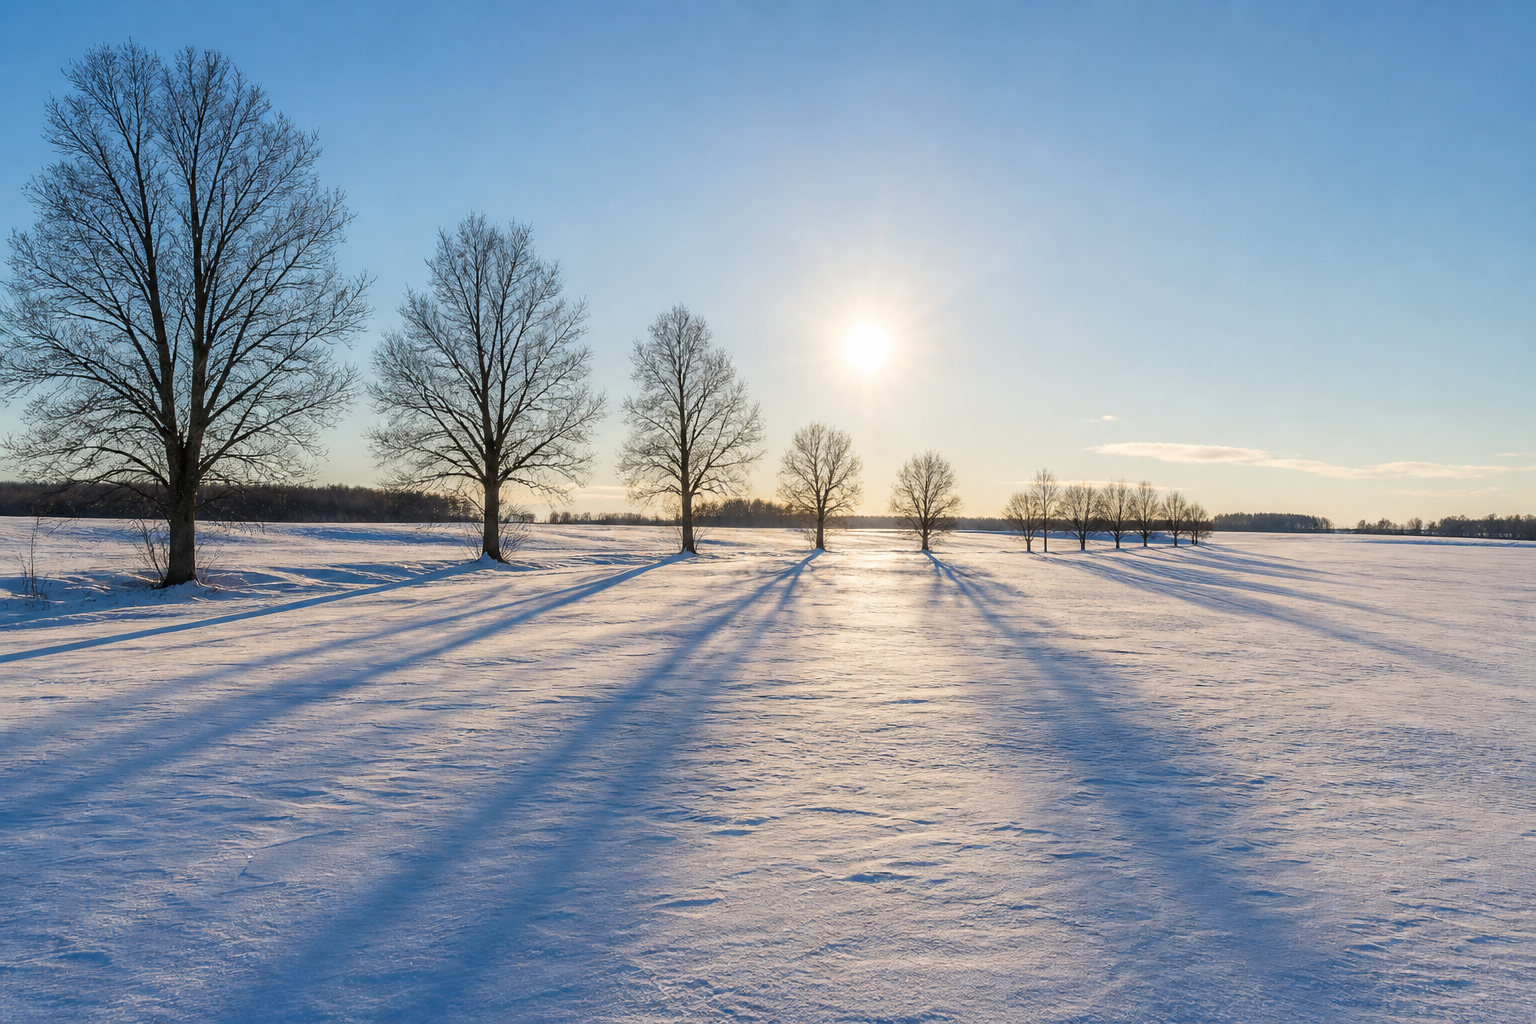
\includegraphics[width=0.58\linewidth]{images/book1/ai/g3-seasons-winter-sun.png}

{\small ظهر شتوي: تبقى الشمس منخفضة، ويأتي \omterm{def:g1:light-and-shadows:source}{الضوء} مائلًا، وتمتدّ الظلال طويلة على الثلج.}
\end{omfigure}

\section{تمارين}

\begin{exercise}[$\star$]\label{exo:g3:sun-days-seasons:1}
في أيّ فصل من \omterm{def:g3:sun-days-seasons:year}{فصول السنة} يكون قوس الشمس أعلى وأطول؟ وفي أيّها
يكون أخفض وأقصر؟ وماذا يفعل ذلك بطول النهار؟
\end{exercise}

\begin{exercise}[$\star$]\label{exo:g3:sun-days-seasons:2}
في أيّ لحظة من النهار يكون \omterm{def:g1:light-and-shadows:shadow}{ظلّ} العمود أقصر؟ وما الذي يميّز \omterm{def:g1:light-and-shadows:shadow}{ظلّ}
الظهر أيضًا، يومًا بعد يوم؟
\end{exercise}

\begin{exercise}[$\star$]\label{exo:g3:sun-days-seasons:3}
يلقي العمود نفسه \omterm{def:g1:light-and-shadows:shadow}{ظلّ} ظهر بطول حذاءين في حزيران وسبعة أحذية في
كانون الأول. اشرح الفرق بطريقَي الشمس.
\end{exercise}

\begin{exercise}[$\star$]\label{exo:g3:sun-days-seasons:4}
كيف تخبر \omterm{def:g3:sun-days-seasons:sundial}{المزولة} بالوقت؟ وممّ صُنع عقربها المتحرّك؟
\end{exercise}

\begin{exercise}[$\star$]\label{exo:g3:sun-days-seasons:5}
في \cref{met:g3:sun-days-seasons:build}، لماذا يجب أن تبقى العصا
في موضع مشمس طوال النهار؟ وماذا يحدث للساعة في الطقس الغائم ---
وفي الليل؟
\end{exercise}

\begin{exercise}[$\star$]\label{exo:g3:sun-days-seasons:6}
كم تستغرق الأرض في دورة واحدة حول الشمس؟ وكم فصلًا يسع في الدورة
الواحدة؟ رتّبها ابتداءً من الربيع.
\end{exercise}

\begin{exercise}[$\star$]\label{exo:g3:sun-days-seasons:7}
كم يومًا في السنة تقريبًا؟ و--- من فصل سابق --- كم ساعة في
اليوم؟ وأيّ رحلة من رحلتَي الأرض تصنع كلًّا منهما؟
\end{exercise}

\begin{exercise}[$\star$]\label{exo:g3:sun-days-seasons:8}
اذكر قرينتين تراهما من نافذتك في أسبوع واحد وتخبرانك أفي وسط
الصيف أنت أم في وسط الشتاء من غير تقويم.
\end{exercise}

\begin{exercise}[$\star$]\label{exo:g3:sun-days-seasons:9}
حين يكون الشتاء حيث تعيش، أيّ فصل يكون عند الأطفال في النصف
البعيد من الأرض؟ وماذا يثبت هذا في حقّ الظنّ القائل ``يأتي
الشتاء لأن الأرض كلها تبتعد عن الشمس''؟
\end{exercise}

\begin{exercise}[$\star\star$]\label{exo:g3:sun-days-seasons:10}
تغرز بستانيّة حصوات ساعة ظلّها في آذار. وفي حزيران لا يعود \omterm{def:g1:light-and-shadows:shadow}{الظلّ}
يلمس الحصوات في الساعات المعلَّمة. أتحرّكت العصا؟ اشرح ما الذي
انحرف، مستعينًا بما في
\cref{ex:g3:sun-days-seasons:shadowlength}.
\end{exercise}

\begin{exercise}[$\star\star$]\label{exo:g3:sun-days-seasons:11}
تستيقظ رحّالة بلا ساعة ولا هاتف، فترى الشمس في أعلى نقطة تمامًا،
وبعد ساعة تجد \omterm{def:g1:light-and-shadows:shadow}{ظلّ} خيمتها أطول من ارتفاع الخيمة. فأيّ ساعة كانت
حين استيقظت تقريبًا، وأهي أقرب إلى وسط الصيف أم إلى وسط الشتاء؟
احتجّ بقاعدة الظهر وبطول \omterm{def:g1:light-and-shadows:shadow}{الظلّ}.
\end{exercise}
